% 2010 年江西卷理科第 10 题：正方体 ABCD-A1B1C1D1（过顶点 A 作与 AB、AD、AA1 成等角的直线）。
% 来源 PDF：普通高考/2010/2010江西理.pdf，SHA-256 994a56c33da151e22af3fabe292d1b5b193866dfc35773a4431e6dfc8a0cc934。
% 原页：第 1 页（A3 三栏）第 2 栏上部，书页码 607。
% 重绘依据：照原页视角，前面为 B-C-C1-B1，后面为 A-D-D1-A1（后脸右上偏移）；
%   不可见棱 A-A1、A1-D1、A1-B1 画虚线。
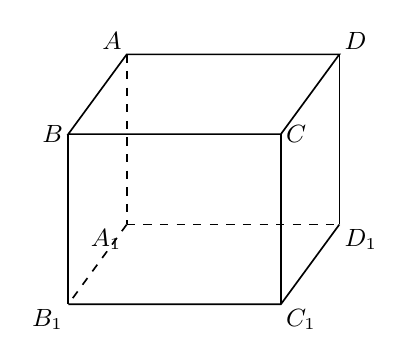
\begin{tikzpicture}[semithick, scale=1.35, every node/.style={inner sep=1.6pt, font=\small}]
  \coordinate (B) at (0,0);
  \coordinate (C) at (2,0);
  \coordinate (C1) at (2,-1.6);
  \coordinate (B1) at (0,-1.6);
  \coordinate (A) at (0.55,0.75);
  \coordinate (D) at (2.55,0.75);
  \coordinate (D1) at (2.55,-0.85);
  \coordinate (A1) at (0.55,-0.85);
  % 可见面与棱
  \draw (A) -- (B) -- (C) -- (D) -- cycle;
  \draw (B) -- (B1);
  \draw (C) -- (C1);
  \draw (D) -- (D1);
  \draw (B1) -- (C1) -- (D1);
  % 不可见棱
  \draw[dashed] (A) -- (A1);
  \draw[dashed] (A1) -- (D1);
  \draw[dashed] (A1) -- (B1);
  \node[above left] at (A) {$A$};
  \node[above right] at (D) {$D$};
  \node[left] at (B) {$B$};
  \node[right] at (C) {$C$};
  \node[below left] at (A1) {$A_1$};
  \node[below right] at (D1) {$D_1$};
  \node[below left] at (B1) {$B_1$};
  \node[below right] at (C1) {$C_1$};
\end{tikzpicture}
